\documentclass{article}
\usepackage{CJKutf8}
\usepackage[T1]{fontenc}
\usepackage[scaled]{beramono}
\usepackage{graphicx}
\usepackage{epsfig}
\usepackage{subfigure}
\usepackage{color}
\definecolor{bluekeywords}{rgb}{0.13,0.13,1}
\definecolor{greencomments}{rgb}{0,0.5,0}
\definecolor{redstrings}{rgb}{0.9,0,0}

\usepackage{listings}
\lstset{language=C,
showspaces=false,
showtabs=false,
breaklines=true,
showstringspaces=false,
breakatwhitespace=true,
frame=single,
escapeinside={(*@}{@*)},
commentstyle=\color{greencomments},
keywordstyle=\color{bluekeywords}\bfseries,
stringstyle=\color{redstrings},
basicstyle=\ttfamily
}
\begin{document}
\begin{CJK}{UTF8}{gbsn}
\title{实验一\\
基于数字信号处理器的系统开发工具}
\author{王亭午,2012011018,无210班}
\date{2015年9月20号}
\maketitle
\section{实验目的}
\subsection{学习软硬件协同设计的系统开发方法和辅助工具}
\subsection{熟悉集成开发和调试环境}
\subsection{掌握利用系统开发步骤和软件开发流程,学会软件调试工具和代码分析工具的使用}
\subsection{掌握系统验证方法和评估系统地使用方法,了解评估系统的基本组成和系统信号通路}
\section{实验材料}
\subsection{实验中使用的集成开发和调试环境软件版本}
美国公司的评估板或软件源程序采用位于的例子工程。
\subsection{实验用配件}
一对标准接口的转和转立体声音频连接线(已配好)耳机。音乐播放器,也可以用机播放音乐。
\section{实验内容}
\subsection{实验一:集成开发环境中的工程建立和代码编译}
\subsubsection{实验步骤} 
a. 运行集成开发环境程序。从开始菜单进入 Analog Device -> VisualDSP++ 4.5-> VisualDSP++ Environment或者点击系统桌面的快捷方式\\
b. 进入菜单 File->New->Project, 弹出 Project Wizard 窗口,填写 Name, Directory. Project Type选择 Standard Application. 注意工程的目录或路径不能使用中文名称。\\
c. 选择 Processor Types 为 ADSP-BF533\\
d. 对于 ldf 和 startup code, 先选择不添加,后选择添加,看有什么异同,理解 ldf 的用途\\
e. 添加测试样例源代码。在工程选单上右击鼠标,弹出"Add File(s) to Project..", 添加源文件。
以 fir 的样本程序为例:fir.asm 为 FIR 函数的汇编语言实现,fir\_test.c 为 C 语言的调
用主程序; filter.h 为宏 和 函数定义头文件; fir\_coeff.h 为系数定义头文件; fir\_input.h 为
输入数据头文件;mds\_def.h 为系统常量和数据类型定义头文件;tfilter.h 为函数原型定义和
测试错误定义头文件。\\
f. 编译源程序构建工程。在工程选单上右击鼠标,弹出"Build Project", 进行编译和构建。新的软件版本中,系统
会默认 ldf 文件。如果编译成功,系统会自动加载编译好的代码,并且断点停留在第一条执
行语句处。此时就可以运行程序。\\
g. 运行程序。此时可以使用单步执行或者设置断点等。分别尝试菜单的 step over (单步通过), step into(单步进入函数), 或者 run(执行)等的模式。
\subsubsection{实验问题}
\subsubsection*{问题 1.1: “ldf”和 “startup code”两个文件在集成开发环境中起什么作用?是必不可少吗?}
答案:ldf全称为,即链接描述文件。ldf是用来设置存储区资源分配的文件,是必不可少的。
如果我们不添加文件。则是由系统直接连接处理器配备的文件。
第二个文件则是用来初始化并且配置处理器状态的,包括了和编译器配置等初始选项。
在标准运行模式下,这个文件也是必不可少的。
\subsubsection*{问题 1.2: 请浏览每个源文件的内容,从 fir\_test.c 的 main 函数进入,各个函数的调用流程是怎样的?}
答案:这其实是一个最为简单的项目结构,在头文件和初始化代码中有一些声明。
进入fir\_test.c 的 main 函数后,首先进行了一些必要的变量声明;此后调用fir\_init(s, h, delay, tapLength)进行初始化。
最后调用函数的主体部分被调用:fir(IN, OUT, nsamples, \&s) 
对于输入信号进行滤波处理,生成输出信号。这是一个FIR滤波器。
\subsection{任务二:使用代码分析工具查看仿真结果和分析代码性能}
\subsubsection{实验步骤} 
a. 点击 Tool->linear profiling->new profile, 创建新的特性统计窗口。\\
b. 选择 project->rebuild project ,重新执行程序,可以看到统计不同的执行时间百分比\\
c. 点击 View->Debug Window->Expressions,弹出表达式调试窗口,双击空白内容,
填写“IN”,观察数组 IN 的内容;再填写“OUT”,观察输出结果的数值。\\
d. 使用 PLOT 工具。点击 View->Debug Window->plot->new... 然后填写相关内容。其中 Address
需要用 Browse 按钮,从列表中选择相对应的数组或者指针地址。Count 选择 260 (input 数组大小),
类型选择 short,其他的选项可以尝试一下。之后软件会自动绘制数组的波形图。请观察 IN,OUT 数组波形图,并且对比滤波前后的效果。\\
我们的到的结果图如下:
\begin{figure}[th]
\begin{minipage}[t]{0.5\linewidth}
\centering
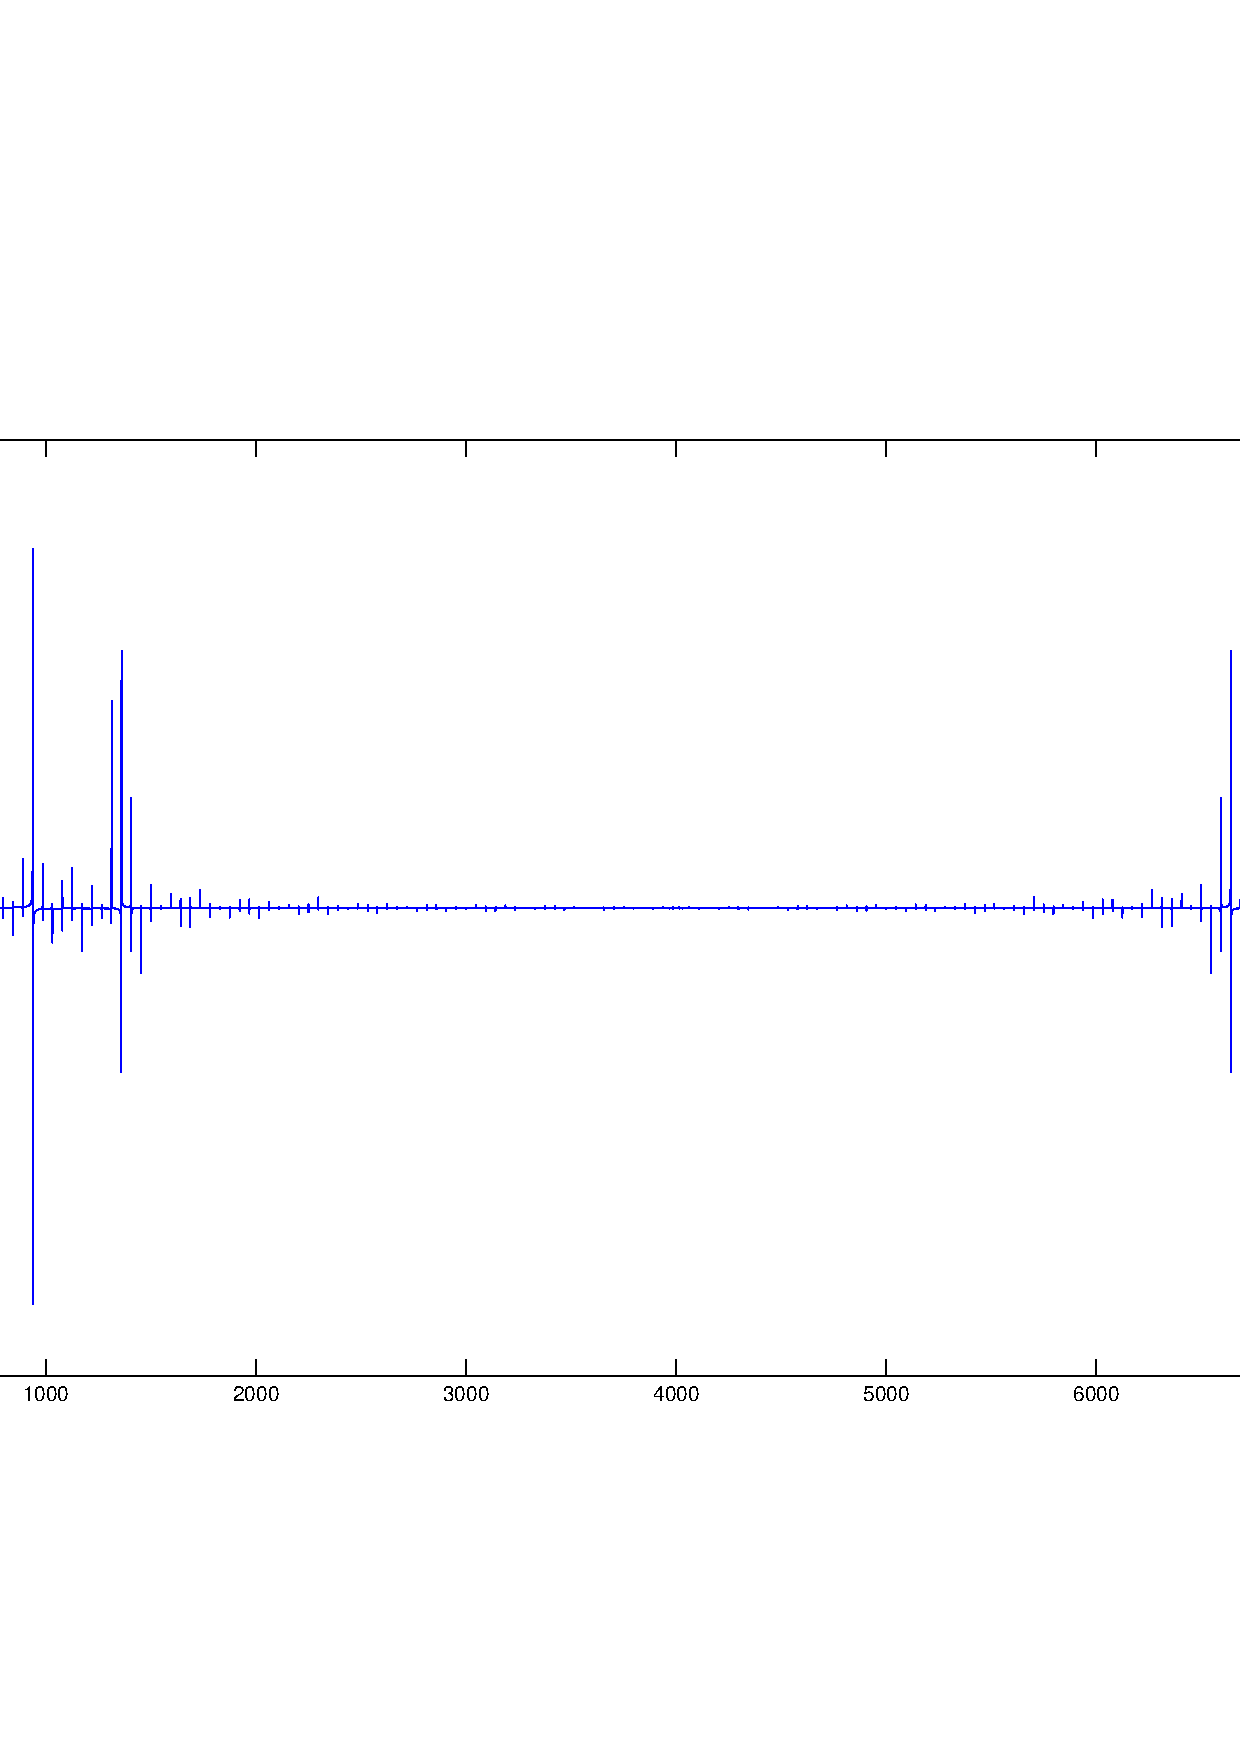
\includegraphics[width=2.2in]{2.jpg}
\caption{观察IN,OUT数组内容示范}
\end{minipage}%
\begin{minipage}[t]{0.5\linewidth}
\centering
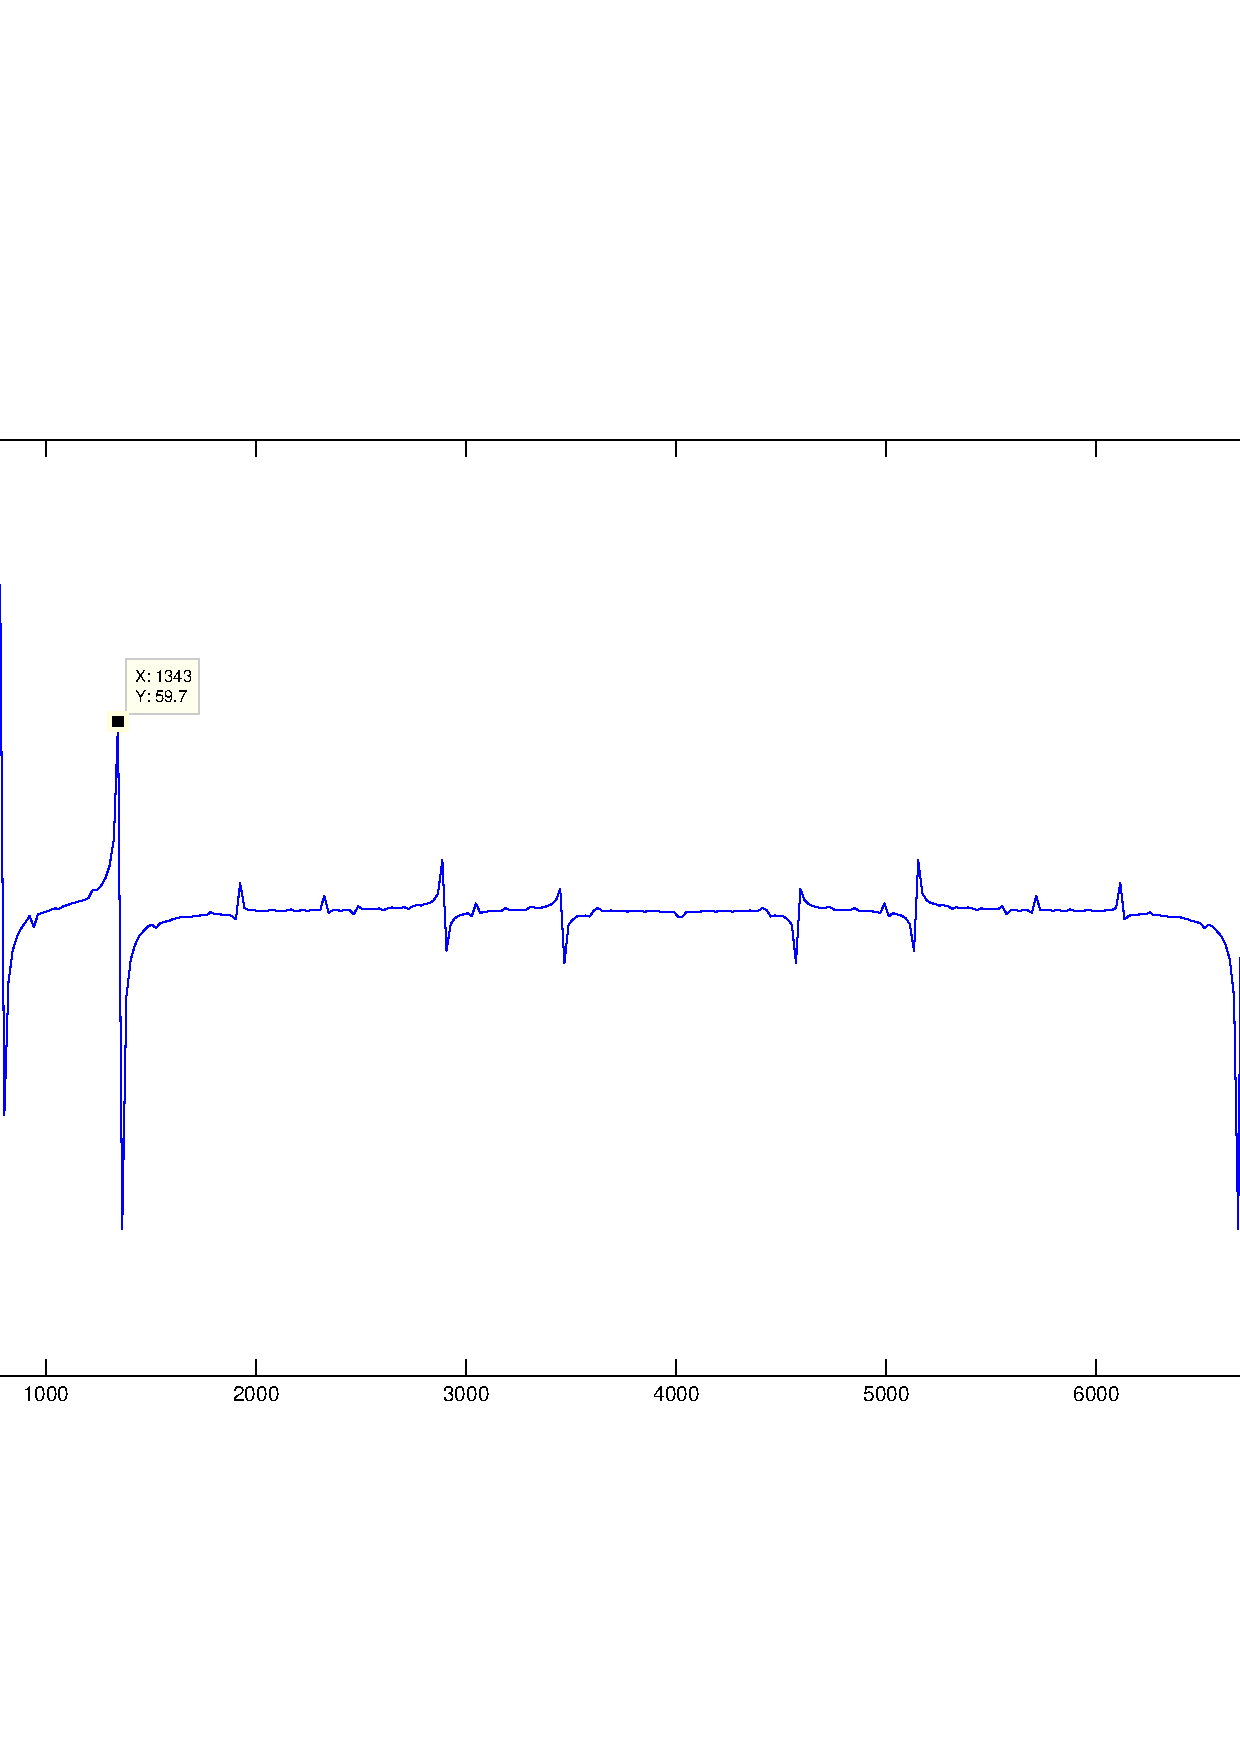
\includegraphics[width=2.2in]{2_2.jpg}
\caption{不同的执行时间百分比}
\end{minipage}
\end{figure}
\begin{figure}[h]
\begin{minipage}[t]{0.5\linewidth}
\centering
\includegraphics[width=2.2in]{3.jpg}
\caption{运行前IN,OUT数值}
\end{minipage}%
\begin{minipage}[t]{0.5\linewidth}
\centering
\includegraphics[width=2.2in]{4.jpg}
\caption{运行后IN,OUT数值}
\end{minipage}
\end{figure}
答案:可以从Fig. 1中看到,我们的可以在表达式调试窗口中看到我们的结果。
在我们运行程序之前,我们的OUT变量都还是0,在运行之后,会得到我们滤波之后的值。\\
从Fig. 2我们可以看到不同的执行时间百分比。
\subsubsection{实验问题}
\subsubsection*{问题 2.1: Linear profiling 中的百分数的单位是什么?也就是说,这个百分比的总量是什么?}
答案:Linear profiling 中的百分数的意义是每一段程序运行(可能是编译,也可能是运行)所消耗的时间占整段程序所消耗的时间的百分比。
由于其物理意义是比值,因此其单位为 "1"。他表示的是这个百分比的总量是整段程序运行所耗费的总时间。
在我们第一个图Fig. 2中应该是编译链接的时间。
\subsubsection*{问题 2.2:数组 IN 是在哪里定义和初始化的?观察数值的时候,可以通过什么途径将它的
内容导出到文件中?用数据文件方式导出和导入数据时,对话框中的参数如何选取?用类似的方法,观察 memory 和 register 中的数据。}
答案:数组 IN 是在 fir\_input.h 中定义的。这里的IN是静态变量,所以在编译的时候就进行了初始化。
可以通过memory栏中的dump选项将内容导出到dat文件中。
在以数据文件方式进行导入导出的时候,
我们在对话框中可以根据用户需要选取数据类型、数据显示的进制以及导入或导出的数据的个数count。这些根据我们的具体情况来决定。
\subsubsection*{问题 2.3:在“Plot Configuration”窗口中,“data”选项中的数据类型的选择依据是什么?
举例说明。输入输出的 fract16 类型等效于 C 编译环境中的哪种数据类型?(可以请教帮助系统)。}
答案:选择的依据是我们到底用的是什么样的数据。
在头文件mds\_def.h中,
short类型被定义为fract16,等效于short。所以我们也这样选择。
\subsubsection*{问题 2.4: 用“plot”工具做频谱分析时,配置参数该如何选取?展示输入、输出的时域和频域波形,分析该滤波器的幅频特性。(参看课件中的代码分析工具“DSP memory plot”中的图示)。}
答案:我们选择信号 IN 的长度的260,数据类型选择 short。如图:
\begin{figure}[h!]
\centering
\includegraphics[width=4.2in]{5.jpg}
\caption{频域波形}
\end{figure}
从频域响应不难看出,此滤波器为低通滤波器。
\subsubsection*{问题 2.5:“OUT”存在什么地方?用什么方法可以以文件的形式导出该组数据?}
答案:OUT是定义了的全局变量。具体存在0xff800680开头的内存空间。
可以通过memory->dump的方式将其以文件形式导出。
\subsubsection*{问题 2.6:打开 fir.asm,观察这个汇编代码和你学过的汇编代码的指令格式有什么不同?
你如何评价这种汇编指令格式?}
答案:指令更加多,支持运算符操作的寄存器级指令,比我们以前学的难,开发起来应该更加方便。
\subsection{任务三:仿真过程中的错误调试和解决}
错误调试和解决是进行任何程序设计的基本要求,在 DSP 的系统设计中,尤其重要和有难
度,因为 DSP 程序设计本身比通用处理器需要更加的了解系统结构和资源状况,并且需要有效
的利用特殊的处理单元,这就对查错和调试本身提出了更高的要求。此次实验进行简单的错误调
试和解决。
\subsubsection{实验步骤}
a. 在前面建立的工程中,将 fir\_test.c 的第 13 行\#include "fir\_coeff.h" 注释掉,进行编译。\\ 
b. 此时系统会报错,主要是未定义的错误,这个在忘记定义或者未包含头文件的情况下会经常发生。自己尝试将源程序中的程序行改成错误的形式,尝试编译。\\
c. 调试选项比较
\subsubsection{实验问题}
\subsubsection*{问题 3.1: 显示的错误识别代码(identification code)是什么?怎么能够通过此代码快速查
找到详细的错误描述和处理建议?如何处理该错误?}
\begin{figure}[h!]
\centering
\includegraphics[width=4.5in]{6.jpg}
\caption{错误结果}
\end{figure}
在这段错误说明中,我们发现了两个错误识别代码cc0020,cc3089。打开help截面,根据帮助,解决方案建议分别是:
“根据编译器报错的详细信息进行修改”, “确保在使用某变量前已进行定义”。
\subsubsection*{问题 3.2: 记录实验中发生的至少三种典型错误,并描述错误原因及解决方法。}
答案:\\
错误一:
cc0175:warnings, subscript out of range。这是数组越界访问的错误。\\
错误二:
cc0101∶error∶"i" has already been declared in the current scope。已经声明过的变量被重定义
我们的解决方法:不要重定义变量。\\
错误三:
cc0065:error:expect a ";"
这是漏写分号的错误。
\subsubsection*{问题 3.3:在对于Blackfin533处理器的simulator,存在两种可选的Session,一种为single
processor simulator,第二种为“Blackfin family complied \\simulator”,这两者有什么区别呢?
在实验中选择不同的simulator,比较其特点。} 
答案:具体的原理比较复杂,区别在于解释的方式。
前者每次只解释一条指令,而另外一个.dxe文件构建为.exe文件,再将其整体加载到Simulator中,这可以提高仿真的速度。
\subsection{任务四:评估板模块连接和检测}
[注意] 请不要用手触摸裸露的电路板或者元器件,移动电路板时,请尽量握住电路板绝缘
部分的边缘和坚固的支架器件。
对照评估系统套盒手册( ADSP − BF56xx EZ − KIT Lite Evaluation System Manual )中的说明和电路原理图,
找到 SW4 ( BF561 )、 SW9 ( BF533 )和 SW10 ( BF561 )、SW1 ( BF533 )的位置,下面的步骤会用到。
找到音频接口下面( PCB 板背面)的拨码开关 SW10 ( BF561 )或 SW1 ( BF533 ),
将 PIN − 1拨向 PIN − 12 , PIN − 2 拨向 PIN − 11 。 SW10 是 Audio Loopback 开关,用于自检测。
等检测步骤完成后,请将 SW10 ( BF561 )或 SW1 ( BF533 )位置还原。
\subsubsection{实验步骤}
a. 连接立体声音频信号接口。
将 PC 机(或任意音频播放机)耳机插孔与评估板的音频输入( Audio in )插孔用音频线连接起来,
将音频输出口与耳机相连。实验中使用的是 RAC to 3.5mm stereo cable 音频线,注意 RAC 接口的颜色对应关系。
本次实验使用任意的音频输入口,前 2 个音频输出口。在直通实验中,如图 1 所示,输入口1 的数据默认会被发送到输出口 1,输入口 2 的数据默认会被发送到输出口2。
一般的BF533 − EZkit 可以按照图 1 所示连接。有些 BF561 − EZkit 可能要要换到第二个插孔,
因为批号不同,所以需要在运行程序时,通过变换插孔确认。\\
b. 接通开发板电源\\
c. 检测控制接口。
当接通电源后,评估板的流水灯通常会处于一个流水闪烁的状态,这是复位之后的默认程序,
表示系统在一定程度上工作正常。\\
d. 检测音频接口。
播放音乐,用耳机试听。如能听到正常的音乐声,证明使用的音频输入输出设备和接口正常。
\subsubsection{实验问题}
\subsubsection*{问题 4.1: 你选用的评估板型号和序号是什么?版本号( REV )是多少?}
答案:选用的评估板型号为 BF553-EZLITE,REV=1.6。因为板子已经被收回去了,我不记得序号了。
\subsubsection*{问题 4.2: 电路板上有很多元器件,你能认出几种?各有什么功能?}
答案:我可以认出来的有:\\
第一类:处理器、存储器,这是冯诺依曼体系中最重要的部分,主要用于计算,控制与存储。\\
第二类:基本电路元件:电阻、电容、晶振。他们用来完成实现,支持板子的工作。\\
第三类:IO接口和供电口:用来烧录,供电和输入输出。
\subsubsection*{问题 4.3: 请在帮助系统中查阅 EZ − kit 手册中的电路原理图,解释为什么这样能检测音频接口设备工作正常?}
答:这个时候,音频型号相当于直接连到输出端口。如果能成功听到音乐,就可以说明接口正常。
\subsection{任务五:系统验证——运行立体声音乐直通例程Talk−Through}
这个程序主要完成立体声音频信号的实时采集和实时播放。立体声信号通过 Audio in 插口输
入评估板,经 ADC ( AD1836 )采样后通过 DMA2\_0 输入 BF561 , BF561 对信号进行存储
和处理后,通过 DMA2\_1 通道发送回到 DAC ( AD1836 )将数字信号变成模拟立体声信号
输出,通过连接在 Audio out 插口的耳机可以听到播放的音乐。
\subsubsection{实验步骤}
BF561EZ − Kit 的 SW4 的拨码开关,对应于\(I^2S\)的工作模式,应该是5和6位置处于 ON 的状态,用于时钟和帧同步。\\
a. 评估板与 PC 连接。
用仿真数据连接线( USB )将 PC 机 USB 接口和评估板 USB 接口连接起来。\\
b. 建立 session。
建立相应的链接 session ,激活。\\
c. 建立工程,导入源程序,导入 Talk\_Through\_561\_I2S 工程文件。\\
d. 播放音乐文件,编译工程并加载运行打开音频播放机,运行程序。从输出的耳机中可以正常听到音乐声。
\subsection{任务六: 实时音频信号处理 — “和/差”立体声处理}
在音频压缩编码中,为提高立体声信号压缩效率,常常利用立体声信号之间的相关性,
将两声道之和作为主声道(main channel)编码,而两声道之间的差值作为边信息(side-information)编码,
这种技术被称为和/差(M/S)立体声处理。
\subsubsection{实验步骤}
a. 新建一个 C 程序,可命名为“Process\_data\_MS.c”,
仿照 Talk-Through 工程文件中的源程序 Process\_data.c 编写“和/差”(M/S)立体声处理\\
b. 建议不改变 4 个输出和 4 个输入变量名,增加对应的 4 个临时变量, 对应“和”声道
为 iM0 和 iM1, “差”声道为 iS0 和 iS1,并计算输入信号之“和/差”。
将自己编写的 Process\_data\_MS.c。
加入Talk-Through工程,注意添加相应的变量声明、
函数声明和调用。重新编译工程,并运行程序。此时请分别播放实验指导书压缩包中附带的音乐文件。\\
\begin{lstlisting}
void Process_Data(void) {
	int iM0 = iChannel0LeftIn + iChannel0RightIn;
	int iS0 = iChannel0RightIn - iChannel0LeftIn;
	iChannel0LeftOut = iM0;
	iChannel0RightOut = iS0;
	
	int iM1 = iChannel1LeftIn + iChannel1RightIn;
	int iS1 = iChannel1RightIn - iChannel1LeftIn;
	iChannel1LeftOut = iM1;
	iChannel1RightOut = iS1;
}
\end{lstlisting}
我们修改了我们的代码如上面所示,通过运行之后我们的代码成功了。
\subsubsection{实验问题}
\subsubsection*{问题 6.1:你能听出左右声道有什么区别吗?你能发现这样处理还可以有什么应用吗?}
答案:(1)声音的大小有区别。左声道为和声道,因此声音很大;而右声道为差声道,声音较小。
(2)左声道是音乐,右声道人声比较明显。\\
这样的处理有着十分广泛的应用。
分成两路传输之后,两路信号作差实现噪声相消,恢复出清晰的人声,提高通话的质量。同时也可以只传差声道节省带宽。
\subsection{任务七:系统功能分析Talk\_Through例程分析}
1. 数据通路:\\
使用通道 SPORT0 进行数据传送,包括数据接收和发送,启动两条 DMA 通道,分别接收和发送数据。\\
2. 工作过程:\\
数据从 AD1836 进行采样,然后经过 SPORT0 通道使用 DMA1@BF533 或 DMA2\_0@BF561
存放于读入缓存器 iRxBuffer1,同时触发一次中断响应,相应端口输入数据被读入到对应的存储器地址空间:
\begin{lstlisting}
iChannel0LeftIn = iRxBuffer1[INTERNAL_ADC_L0];
iChannel0RightIn = iRxBuffer1[INTERNAL_ADC_R0];
iChannel1LeftIn = iRxBuffer1[INTERNAL_ADC_L1];
iChannel1RightIn = iRxBuffer1[INTERNAL_ADC_R1];
\end{lstlisting}
此时调用 processdata()处理数据,然后将数据写入输出数据对应的存储器地址空间
iChannel0LeftOut,iChannel0RightOut,iChannel1LeftOut和
iChannel1RightOut,
这些变量又被转入发送缓存器 iTxBuffer1,
同时通过 DMA2@BF533 或 DMA2\_1
@BF561 发送到 1836 的相应 DA 通道,转换成模拟声音输出。
\begin{lstlisting}
iTxBuffer1[INTERNAL_DAC_L0] = iChannel0LeftOut;
iTxBuffer1[INTERNAL_DAC_R0] = iChannel0RightOut;
iTxBuffer1[INTERNAL_DAC_L1] = iChannel1LeftOut;
iTxBuffer1[INTERNAL_DAC_R1] = iChannel1RightOut;
\end{lstlisting}

\subsubsection{实验问题}
\subsubsection*{问题 7.1:分析程序的整体结构,程序由几部分组成,各完成什么功能?
音频信号从模拟输入到模拟输出经过了哪些“路径”?}
答案:程序的组成由初始化函数、和数据处理函数组成。
主程序首先调用各个的初始化函数,从输入端口对模拟音频信号进行采样,结果被存到我们的iRxBuffer1内存空间中,同时触发中断。
这个时候我们的数据处理部分读取到数据进行处理,然后写入存储器,再转入缓存器中。
最后发送至端口相应的 DA 通道,转换成模拟声音输出。
\subsubsection*{问题 7.2:初始化函数具有通用性吗?为什么?}
初始化函数具有部分通用性。初始化函数是对DSP板上的元件设置和选择的过程。
如果我们使用的功能需要不同的元器件和设置,就可以通过修改初始化函数来做到。
\subsubsection*{问题 7.3:SPI、SPORT、DMA 的操作代码和配置代码都在哪里可以看到?
每个代码大体的作用是什么?}
在Initialize.c中。
SPI设置对应我们1836的配置;SPORT0配置对应于1836间的数据交换。
DMA1,DMA2两个端口的设置负责SPORT0与BF533的数据交换。
\section{总结问题}
\subsection{IDDE有什么功能?}
答案:集成开发和调试环境(IDDE)的功能有以下几个方面:\\
调试功能,绘图功能;源文件编辑;工程管理;代码产生;工程编译链接选择;VDK 功能:从软件中获取硬件实现详情;工作空间管理;开发功能;
\subsection{Simulation, emulation 和 evaluation 的目的是什么?分别使用什么工具?}
答案:simulation是软件仿真,而emulation是硬件仿真,evaluation是硬件评估。\\
simulation使用IDDE和软件simulator。emulation使用的EZICE和In Circuit Emulator。
而evaluation使用评估板。
\subsection{简述 DSP 开发流程和软件建立过程。}
答案:\\
1. 建立一个工程(Create a project)\\
2. 配置工程选项(Configure project options)\\
3. 添加和编辑工程源文件(Add and edit project source files)\\
4. 定义工程构建选项(Define project build options)\\
5. 构建调试版本的工程(Build a debug version (executable file) of the project)\\
6. 建立一个调试平台加载可执行文件(Create a debug session and load the executable)\\
7. 运行和调试程序(Run and debug the program)\\
8. 构建一个执行版本的工程(Build a release version of the project)\\
\subsection{谈谈帮助系统在学习 DSP 开发中的作用和你的体会。}
答案:我个人觉得就是DSP中的matlab的help,基本上功能已经非常强大了。
比起直接使用google的话,针对性更加强,更容易找到答案。不过个人认为复杂的问题,还是得上google。
\subsection{本次实验中遇到的主要问题和收获,对课程和实验的建议等。}
答案:本次实验遇到了一个非常有意思的问题,那就是如果我们在头文件里面申明一个external int,
我们在process\_data的时候,使用这个申明的变量是会出问题的。
但是奇怪的是,其他的同样方法申明的变量确是可以访问的。和助教老师调了一段时间,都没办法搞定。最后是在process\_data里面申明临时变量解决问题的。希望老师可以给出这个问题的原因解答。\\
此外,最大的建议就是希望可以转到ubuntu平台或者WIN 7平台。现在跑去实验室才能调试,感觉带来很多的不便。




\end{CJK}
\end{document}

enter image description here
